\documentclass[11pt, oneside]{article}
\usepackage[letterpaper, margin=2cm]{geometry}
\usepackage{MATH566}
%\usepackage{sagetex}

\begin{document}
\noindent \textbf{\Large{Caleb Logemann \\
MATH 566 Discrete Optimization\\
Midterm I
}}

%\lstinputlisting[language=Sage]{03_2.sage}
\begin{enumerate}
  \item % #1 Done
    Suppose you are making a schedule for an airport.
    There are $n$ arriving flights.
    Every airplane $j$ has a possible time arrival  in interval $[a_j,b_j]$
    (plane can fly faster or slower).
    Determine the actual arrival schedule for each airplane such that the
    smallest gap between consecutive flights is maximized
    and for all $j$, airplane $j$ arrives before $j+1$.
    Formulate a linear program that solves the problem.

    \emph{
      (Example: Suppose there are three airplanes. They have arrival intervals $[1,5],[2,7],[6,7]$.
      Then we can assign arrival times to the airplanes, for example $2,4.5,6.2$. The smallest
      gap in this schedule is $1.7$ between the second and third airplane. The number $1.7$
      is the number we want to maximize. Notice that we do not allow schedule $4,2,7$, where the first
      airplane arrives AFTER the second one although the it would be feasible with respect to $[a_i,b_i]$s
      (it is easier to solve if the order is fixed).)
    }

    First I will define a new set of variables, $t_j$ for $1 \le j \le n$, to
    be the time that plane $j$ arrives at the airport.
    Clearly we must have the constraints
    \begin{align*}
      t_j \ge a_j \\
      t_j \le b_j
    \end{align*}
    for all $j$, such  that $1 \le j \le n$.
    These constraints force each plane to arrive inside of the allowed interval
    $\br{a_j, b_j}$.
    Also if the order that the planes arrive is to be enforced, the constraints
    \[
      t_{j+1} - t_{j} \ge 0
    \]
    are required for $1 \le j \le n-1$.
    Lastly we need to set the objective function for this linear program.
    Our objective function needs to maximize the smallest time gap
    $t_{j+1} - t_j$ or in other words
    $\max* \min*_{1 \le j \le n-1}\p{t_{j+1} - t_j}$.
    I am going to create another variable $m$ to be this minimum value, that is
    \[
      m = \min*_{1 \le j \le n-1}\p{t_{j+1} - t_j}
    \]
    In this case the objective function just becomes $\max* m$.
    However we need constraints to insure that $m$ does in fact equal the
    minimum value.
    I will use the following constraints
    \[
      m \le t_{j+1} - t_j
    \]
    for all $j$ such that $1 \le j \le n-1$.
    These constraints guarantee that
    \[
      m \le \min*_{1 \le j \le n-1}\p{t_{j+1} - t_j}.
    \]
    With the addition of the objective function maximizing $m$, we will achieve
    equality.
    Therefore the entire linear program that solves this problem is
    \[
      (P) =
      \begin{cases}
        \text{maximiz}    & m \\
        \text{subject to} & t_j \ge a_j         \quad 1 \le j \le n \\
                          & t_j \le b_j         \quad 1 \le j \le n \\
                          & t_{j+1} - t_j \ge 0 \quad 1 \le j \le n-1 \\
                          & m \le t_{j+1} - t_j \quad 1 \le j \le n-1 \\
      \end{cases}
    \]
    Note that there is no minimum value of $m$ and we aren't enforcing
    nonnegativity to the variables $t_j$ as the intervals $\br{a_j, b_j}$
    supersede these conditions.

  \item % #2 Done
    Solve the following linear program $(P)$ using simplex method.
    \[
      (P) =
      \begin{cases}
        \text{maximize}    &x_1+x_2 \\
        \text{subject to}  & x_1 \leq 1 \\
                           & -x_1 + x_2 \leq 1 \\
                           & x_1,x_2 \geq 0
      \end{cases}
    \]
    Check your solution using computer program (APMonitor, Sage,\ldots).
    Plot the set of feasible solutions and mark the optimum.
    Solving using simplex method means make the sequence of simplex tables.

    First I will solve this problem using the simplex method.
    First I will introduce slack variables so that the new linear program is
    \[
      (P) =
      \begin{cases}
        \text{maximize}    &x_1+x_2 \\
        \text{subject to}  & x_1 + x_3 \leq 1 \\
                           & -x_1 + x_2 + x_4 \leq 1 \\
                           & x_1,x_2,x_3,x_4 \geq 0
      \end{cases}
    \]
    The initial basic feasible solution for this linear program is
    \begin{align*}
      x_3 &= 1 - x_1 \\
      x_4 &= 1 + x_1 - x_2 \\
      z &= 0 + x_1 + x_2
    \end{align*}
    First $x_1$ can be increased by $1$.
    \begin{align*}
      x_1 &= 1 - x_3 \\
      x_4 &= 2 - x_2 - x_3\\
      z &= 1 + x_2 - x_3
    \end{align*}
    Next $x_2$ can be increased by $2$.
    \begin{align*}
      x_1 &= 1 - x_3 \\
      x_2 &= 2 - x_3 - x_4\\
      z &= 3 - 2x_3 - x_4
    \end{align*}
    Now all of the coefficients of the variables in the objective function
    are negative so this is the optimal solution.
    The optimal solution is $x_1 = 1$, $x_2 = 2$, and $z = 3$.

    Next I will check this solution using sage.
    The following script solves this linear program.
    \lstinputlisting[language=Sage]{midterm_2.sage}
    The following is the output of this script.
    \begin{verbatim}
      Objective Value: 3.0
      x_1 = 1.0
      x_2 = 2.0
    \end{verbatim}

    Lastly I will show a plot of the feasible region, along with the optimal
    solution and the path that I took in the simplex method to get there.
    \begin{center}
      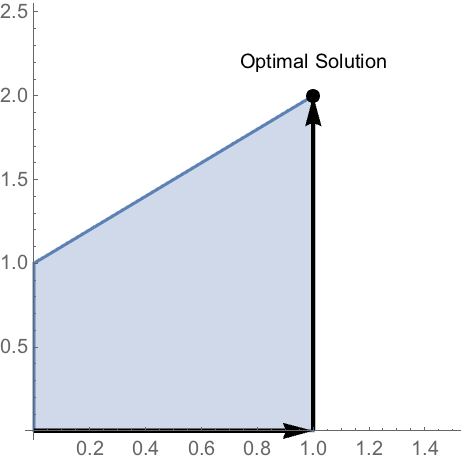
\includegraphics[scale=.5]{Figures/midterm_3.png}
    \end{center}

  \item % #3 Done
    Consider the following algorithm. Input is a connected graph $G=(V,E)$ and
    a cost function $c:E \rightarrow \mathbb{R}$.
    Start with $H$ being a copy of $G$.
    First, the edges $E$ are ordered such that
    $c(e_1) \geq c(e_2) \geq \ldots \geq c(e_m)$.
    Then process edges one by one according to the ordering.
    Processing edge $e_i$ means looking if $H-e_i$ connected.
    If $H-e_i$ is connected, then $e_i$ is removed from $H$.
    Otherwise $e_i$ is kept in $H$.
    After all edges are processed, the resulting $H$ is the output.
    Now you can pick what to do.
    Either a) or b):
    \begin{enumerate}
      \item[(a)]
        Implement the algorithm and use as inputs the same graph we used for the minimum spanning tree
      \item[(b)]
        Prove that the algorithm produces minimum spanning tree.
    \end{enumerate}

    I chose to do part (a).
    The following script creates random graphs and implements the given
    algorithm in the function minimumSpanningTree.
    \lstinputlisting[language=Sage]{midterm_3.sage}
    This function requires a breadthSearchFirst algorithm which I implemented
    as follows.
    \lstinputlisting[language=Sage]{breadthFirstSearch.sage}
    This function checks to see if a graph is connected.
    If a graph isn't connected it will return with an infinite
    distance from the root vertex to some other vertex.

    The following two plots are the results on running the initial script twice.
    They show that the algorithm does in fact find the minimum spanning tree.
    \begin{center}
      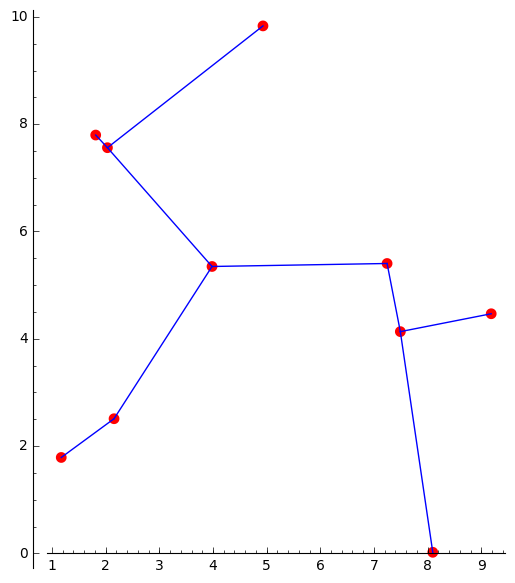
\includegraphics[scale=.6]{Figures/midterm_1.png} \\
      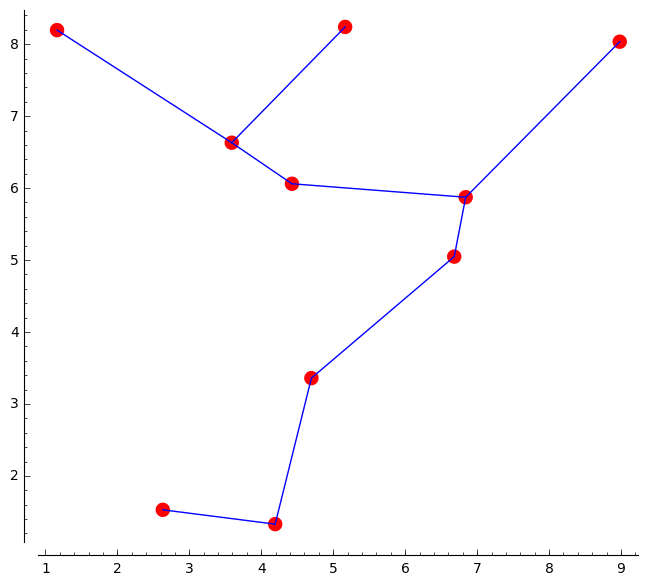
\includegraphics[scale=.5]{Figures/midterm_2.png}
    \end{center}

  \item % #4 Done
    Consider the following problem.
    Input is a connected graph $G=(V,E)$ and a cost function $c:E \rightarrow \RR$.
    Let $T$ be a spanning tree of $G$. The cost of $T$ is defined as the largest cost of an edge
    in $T$:
    \[
      c(T) = \max*\{c(e): e \in E(T)\}.
    \]
    Problem is to find a minimum spanning tree with respect to $c$\\
    Do both a) and b):
    \begin{enumerate}
      \item[(a)] % Done
        Formulate the problem using integer programming

        Let $\set{x_e}$ be a set of binary variables where $x_e$ corresponds to
        whether $e \in E(T)$, the alternative minimum spanning tree, for every edge,
        $e \in E$.
        Let $n = \abs{V}$ and $m = \abs{E}$.
        First note that the alternative minimum spanning tree must be a spanning
        tree, so the constraints associated with a spanning tree must also be
        associated with this alternative spanning tree.
        Namely this implies that $T$ must have $n - 1$ edges or
        \[
          \sum{e \in E}{}{x_e} = n - 1
        \]
        Also $T$ must not contain any cycles.
        This can be expressed with the constraints
        \[
          \sum{e \in E(G[X])}{}{x_e} \le \abs{X} - 1 \quad \forall \emptyset \neq X \subset V
        \]

        Lastly we need to add the objective function.
        The objective function is trying to minimize the maximum cost edge in
        $T$ or
        \[
          \min* \max*_{e \in E}{x_e c(e)}
        \]
        I will create a new variable $m$ to represent the maximum cost of an
        edge in $E(T)$, that is
        \[
          m = \max*_{e \in E}{x_e c(e)}
        \]
        Now in order to enforce this equality certain constraints are needed.
        First $m$ must be larger than any single cost of an edge in $E(T)$.
        This requires the constraints
        \[
          m \ge x_e c(e)
        \]
        for all $e \in E$.
        This makes $m$ larger than $c(e)$ only if $e \in E(T)$.
        Lastly if we add the objective function $\min* m$, this will force
        equality.
        These are all the constraints that are required, so the full integer
        linear program is
        \[
          (P) =
          \begin{cases}
            \text{minimize}   & m \\
            \text{subject to} & \sum{e \in E}{}{x_e} = n - 1 \\
                              & \sum{e \in E(G[X])}{}{x_e} \le \abs{X} - 1 \quad \forall X \subset V, X \neq \emptyset\\
                              & m \ge x_e c(e) \quad \forall e \in E \\
                              & x_e \ge 0 \quad \forall e \in E \\
                              & x_1 \le 1 \quad \forall e \in E \\
                              & x_e \in \ZZ \quad \forall e \in E 
          \end{cases}
        \]

      \item[(b)] % Done
        Find an algorithm for solving this problem in polynomial time and prove its correctness.

        \begin{proof}
          First I will show that any minimum spanning tree is also an
          alternative minimum spanning tree.
          Let $G = (V, E)$ be a graph with a minimum spanning tree $T$.
          It has been shown previously that if $T$ is a minimum spanning tree,
          then for every $e \in E(T)$, $e$ is a minimum cost edge of the cut between
          the connected components in $T - e$.
          Consider the edge $e_{max} \in E(T)$ such that $c(e_{max}) \ge c(e)$
          for all $e \in E(T)$.
          Therefore $e_{max}$ is the minimum cost edge of the cut between the
          connected components of $T - e_{max}$.
          If $T$ was not a alternative minimum tree, then there would be a
          lower cost edge in the cut between connected components of
          $T - e_{max}$.
          Since $e_{max}$ is the minimum cost edge, this implies that $T$ is
          also a alternative minimum spanning tree.
          Therefore any minimum spanning tree is also an alternative minimum
          spanning tree.
          Clearly not all alternative MSTs are MSTs, but all MSTs are alternative
          MSTs.
          This implies that any algorithm that finds a minimum spanning tree
          also finds an alternative minimum spanning tree.
          Therefore I can pick any algorithm that finds a minimum spanning
          tree in polynomial time as my algorithm.
          Kruskal's algorithm can be implemented in $O(m \log{n})$.
          This is better than $m^2$ so it is certainly polynomial.
        \end{proof}
    \end{enumerate}
\end{enumerate}
\end{document}
